% !TEX TS-program = pdflatex
% !TEX encoding = UTF-8 Unicode

% This is a simple template for a LaTeX document using the "article" class.
% See "book", "report", "letter" for other types of document.

\documentclass[11pt]{article} % use larger type; default would be 10pt

\usepackage[utf8]{inputenc} % set input encoding (not needed with XeLaTeX)

%%% Examples of Article customizations
% These packages are optional, depending whether you want the features they provide.
% See the LaTeX Companion or other references for full information.

%%% PAGE DIMENSIONS
\usepackage{geometry} % to change the page dimensions
\geometry{a4paper} % or letterpaper (US) or a5paper or....
% \geometry{margin=2in} % for example, change the margins to 2 inches all round
% \geometry{landscape} % set up the page for landscape
%   read geometry.pdf for detailed page layout information

\usepackage{graphicx} % support the \includegraphics command and options

% \usepackage[parfill]{parskip} % Activate to begin paragraphs with an empty line rather than an indent

%%% PACKAGES
\usepackage{booktabs} % for much better looking tables
\usepackage{array} % for better arrays (eg matrices) in maths
\usepackage{paralist} % very flexible & customisable lists (eg. enumerate/itemize, etc.)
\usepackage{verbatim} % adds environment for commenting out blocks of text & for better verbatim
\usepackage{subfig} % make it possible to include more than one captioned figure/table in a single float
% These packages are all incorporated in the memoir class to one degree or another...

%%% HEADERS & FOOTERS
\usepackage{fancyhdr} % This should be set AFTER setting up the page geometry
\pagestyle{fancy} % options: empty , plain , fancy
\renewcommand{\headrulewidth}{0pt} % customise the layout...
\lhead{}\chead{}\rhead{}
\lfoot{}\cfoot{\thepage}\rfoot{}

%%% SECTION TITLE APPEARANCE
\usepackage{sectsty}
\allsectionsfont{\sffamily\mdseries\upshape} % (See the fntguide.pdf for font help)
% (This matches ConTeXt defaults)

%%% ToC (table of contents) APPEARANCE
\usepackage[nottoc,notlof,notlot]{tocbibind} % Put the bibliography in the ToC
\usepackage[titles,subfigure]{tocloft} % Alter the style of the Table of Contents
\renewcommand{\cftsecfont}{\rmfamily\mdseries\upshape}
\renewcommand{\cftsecpagefont}{\rmfamily\mdseries\upshape} % No bold!

%%% END Article customizations

%%% The "real" document content comes below...

\title{CS338 HW1}
\author{Brock Ellefson}
%\date{} % Activate to display a given date or no date (if empty),
         % otherwise the current date is printed 

\begin{document}
\maketitle

\section{}

$\frac{1}{3} k(4k^{2}-1) = \frac{1}{3} (2k-1)(2k+1)$


$P(k + 1)= 1^{2} + 3^{2} + 5^{2} + ... (2k-1)^{2} = \frac{1}{3} (2k-1)(2k+1)$


$= 1^{2} + 3^{2} + 5^{2}+....+(2k-1)^{2} + (2k+1)^{2} = \frac{1}{3} (2k-1)(2k+1) + (2k+1)^{2} $


$= \frac{2k+1}{3}[k(2k-1) + 3(2k+1)]$


$= \frac{2k+1}{3}[2k^{2}-k+6k+3]$


$= \frac{1}{3}(k+1) +(2(k+1)-1)(2(k+1)+1)$

\section{}
This is false

$\mid$V$\mid$=2, $\mid$E$\mid$ =7, 

$\mid$F$\mid$ = 2 + 7 - 2 = 7

7 $>$ 4 = 2n 

\section{}

There are two cases:

1: Simple graph is not a cyclic graph therefore u!=v

2: Simple graph is a cyclic graph therefore u=v


Case 1:

 Assumption: A path starting with an odd degree ends with an even degree.
 
 The sum of degrees is 2(Edges)
 
 Therefore, there must be a minimum of one vertex with an odd degree that is a connected component. Being a connected component means that its a pair with each of the vertices.
 
 Therefore, there is always a path from one vertex with an odd degree to another via the connected component 


Case 2: If u is an odd degree, then by the definition of a cyclic graph v must be odd as well

\section{}
\begin{figure}
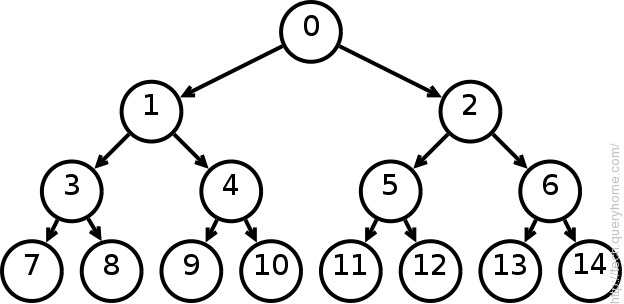
\includegraphics[width=\linewidth]{tree.png}
\end{figure}
Assume that that a binary tree B has n internal nodes and i leaves.

Before proving 

Base Case: B(0): This binary tree only has a root. Since this node has no children, it is, by definition, a leaf. 2(0) + 1 = 1 node.

Induction: B(n): Assuming this tree has $n\geq$ 1 we then know that if will split n into two subtrees n will have a left subtree and a right subtree . This two subtrees will have such a size that l(left subtree) + r(right subtree) + 1(root) = n. The number of leaves on l will be l+1 and the number of leaves on r will be r+1 (we find this by preforming this on B(l) and B(r) and so on until we are only left with the minimum sized subtrees) 


Therefore this means i = l + r + 2. 


Therefore i = n+1.


i + n = total nodes


(n + 1) + n = total nodes 

2n + 1 = total nodes

\section{}

A tree, by definition will only have one path between two nodes.

Therefore, the diameter is that said path between the two nodes

Calling this algorithm on an internal node will return a leaf node, and calling this algorithm on a leaf node will return the node the most far away from the leaf.

This algorithm is correct

\end{document}
